%=================
% Introduction
\chapter*{Introduction}
%=================

This chapter will give a technical introduction to our project.
It will give a concise explanation of the most important terms used in the report.

The first section will briefly explain Wireshark, dissectors and how dissectors are used in Wireshark.
The connection between Wireshark and the Lua structs protocol will also be explained.

The second section will describe how the Lua code works and how it is generated by our utility.

\section*{Wireshark and dissectors}
This section gives a brief introduction to Wireshark and dissectors.
The first part describes what Wireshark is and what it can be used for.
The second part explains exactly what a dissector is, and how a dissector can be used to extend Wireshark.

\subsection*{Wireshark}
Wireshark is a program used to analyze network traffic. A common usage scenario is when a person wants to troubleshoot network problems or
look at the internal workings of a network protocol. An important feature of Wireshark is the ability to capture and display a live stream of packets sent through the network. 
A user could, for example, see exactly what happens when he opens up a website. Wireshark will then display all the messages
sent between his computer and the web server. It is also possible to filter and search on given packet attributes, which facilitates the debugging process.

In \autoref{fig:introshark}, you can see a view of Wireshark.
This specific example shows a capture file with four messages, or packets, sent between internal processes, in other words
it is a view of messages sent by inter-process communication. Each of the packets contain one C struct.
To be able to display the contents of the C struct, Wireshark has to be extended. 
This can be accomplished by writing a dissector for the C struct.

The dissectors can be written in either C or Lua, and in our utility they are written in Lua.
The difference between C and Lua dissectors, and the reason we used Lua is elaborated on in the Pre Study-chapter.
Dissectors, in general, are explained more in detail below.

\begin{figure}[ht]
	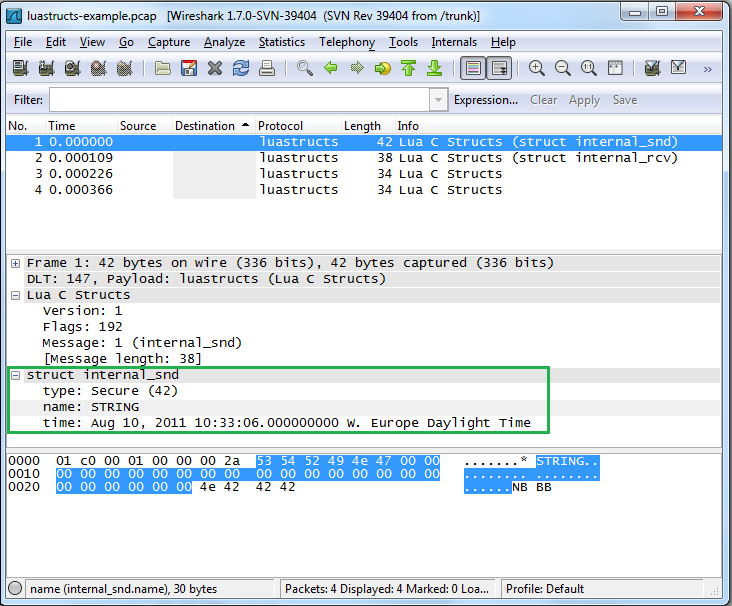
\includegraphics[width=\textwidth]{./img/wireshark_example.png}
	\caption{Wireshark\label{fig:introshark}}
\end{figure}

\subsection*{Dissectors}
In short, a dissector is a piece of code, run on a blob of data, that can dissect the
data and display it in a readable format in Wireshark, instead of the binary representation.

\autoref{fig:introshark} displays four packets, with packet number 1 highlighted.
The content of the packet, a C struct with two members, name and time,  is shown inside the green box.
The dissector takes the C struct, decodes its binary representation and makes it readable by humans.
Without a dissector, Wireshark would just display the struct and struct members as a binary blob.

All the packets containing C structs belong to the protocol called luastructs.
When opening a capture file in Wireshark , this protocol maps the id of the messages to the correct dissector,
and calls them.

\section*{From struct definition to Lua dissector}
This section explains how the Lua dissectors work, and how they can be built by our utility.

The first part explains what happens under the hood of a Lua dissector, while 
the second part is a very brief explanation of how CSjark builds such dissectors.

\subsection*{Lua dissectors}

\autoref{luaexample1} shows what the code for the Lua dissector, displayed in packet 1 in \autoref{fig:introshark}, looks like.
The Proto variable defines a new protocol. In this example, a dissector for the internal\_snd struct, called internal\_snd, is created. 
The different fields of the struct are created as instances of ProtoField, and put in Protocol.fields.
For example, the "name" variable is a string in C, and as such it is created as a ProtoField.string with the 
name "name".

The protocol dissector method is the method that does the actual dissecting.
A subtree for the dissector is created, and the description of the dissector is appended to the information column.
All the ProtoFields are added to the subtree. Here you can see that type, name and time fields are added to the subtree for the internal\_snd dissector.
(The buffer size allocated to the fields is the size of the members in C.)

In the last line the dissector is added to the dissector table as a subdissector for the luastructs protocol.
When running a capture file, where the internal\_snd struct is being sent to another process, it is possible to see the exact contents of the struct, as the example screenshot of Wireshark shows.

\lstset{language=C,caption={Example Lua file},label=luaexample1}
\lstinputlisting[language=C]{./code/luaexample.lua}

\subsection*{CSjark - Automated generation of Lua dissectors}
CSjark is a Python utility that can automatically generate a Lua dissector for 
any valid C header file. It also supports user configuration from files in a specific format.
The C file, in addition to any suitable configuration file, is inputted into a command line interface.
The C file is then sent to the C preprocessor, where C directives are evaluated before the parsing.
The parser creates an abstract syntax tree from the input.
CSjark traverses the abstract syntax tree and finds all the struct definitions.
For every struct that is found, a dissector is generated and written to file.






